\section{Auswertung}
\label{sec:Auswertung}
Für die Auswertung werden Matplotlib \cite{matplotlib}, NumPy \cite{numpy}, SciPy \cite{scipy} 
und Uncertainties \cite{uncertainties} benutzt.

\subsection{Bestimmung der Apparaturkonstante für die große Kugel}
Die Fallstrecke beträgt 
\begin{equation*}
    x = \SI{10}{\centi\meter}.
\end{equation*}
Die Masse, der Durchmesser und die Apparaturkonstante der kleinen Kugel sind:
\begin{align*}
    m_\text{klein} &= \SI{3.71}{\gram} \\
    d_\text{klein} &= \SI{0.0156}{\meter} \\
    K_\text{klein} &= \SI{76.4}{\nano\pascal\cubic\meter\per\kilo\gram}.
\end{align*}
Die Masse und der Durchmesser der großen Kugel sind:
\begin{align*}
    m_\text{groß} &= \SI{4.21}{\gram} \\
    d_\text{groß} &= \SI{0.0158}{\meter}. \\
\end{align*}
Die Dichte des destillierten Wassers beträgt
\begin{equation*}
    \rho_\text{Fl} = \SI{998.2067}{\kilo\gram\per\cubic\meter}.
\end{equation*}
Aus der Masse und dem Volumen der Kugeln ergibt sich jeweils mittels Gleichung \eqref{eqn:dichte}
die Dichte der Kugel:
\begin{align*}
    \rho_\text{klein} &= \SI{1866.39}{\kilo\gram\per\cubic\meter} \\
    \rho_\text{groß} &= \SI{2038.51}{\kilo\gram\per\cubic\meter}.
\end{align*}
Die Falldauern der kleinen und der großen Kugel im Kugelfall-Viskosimeter
bei Raumtemperatur befinden sich in Tabelle \ref{tab1}.
%Daraus besser zwei Tabellen machen?: Nö, denke nicht. Oder wieso meinst du denn?
\begin{table}\caption{Der maximale Drehimpuls $L$, der Gesamtspin $S$ und der Gesamtdrehimpuls $J$ ergeben sich zum Landé-Faktor $g_\text{J}$ für die vier verschiedenen Elemente.}
\label{tab1}
\centering
\sisetup{round-mode = places, round-precision=2, round-integer-to-decimal=true}
\begin{tabular}{S[]S[]S[]S[]} 
\toprule
{$L$} & {$S$} & {$J$} & {$g_\text{J}$}\\
\midrule
5.0 & 1.0 & 4.0 & 0.8\\
0.0 & 3.5 & 3.5 & 2.0\\
6.0 & 1.5 & 4.5 & 0.7272727272727273\\
5.0 & 2.5 & 7.5 & 1.3333333333333333\\
\bottomrule
\end{tabular}\end{table}
\noindent Für die mittleren Falldauern ergibt sich mit den Gleichungen \eqref{eqn:mittelwert} 
und \eqref{eqn:standard}
\begin{align*}
    t_\text{klein} &= \SI{11.7 \pm 0.1}{\second} \\
    t_\text{groß} &= \SI{65.2 \pm 0.3}{\second}.
\end{align*}
Mit Gleichung \eqref{eqn:eta} berechnet sich die Viskosität mit $K_\text{klein}$,
$\rho_\text{klein}$ und $t_\text{klein}$ zu
\begin{equation*}
    \eta = \SI{773 \pm 7}{\micro\pascal\second}.
\end{equation*}
Mit diesem Wert folgt für die Apparaturkonstante $K_\text{groß}$
mittels Gleichung \eqref{eqn:K}
\begin{equation*}
    K_\text{groß} = \SI{11.40(11)}{\nano\pascal\cubic\meter\per\kilo\gram}.
\end{equation*}

\subsection{Bestimmung der Temperaturabhängigkeit der Viskosität von destilliertem Wasser}
Die Falldauern der großen Kugel für verschiedene Temperaturen sind in den Tabellen
\ref{tab2} und \ref{tab3} dargestellt.
%Daraus besser eine Tabelle machen?:
\begin{table}\caption{Das Verhältnis des magnetischen Feldes durch die Beschleunigungsspannung aufgetragen gegen die Höhe.}
\label{tab2}
\centering
\sisetup{round-mode = places, round-precision=2, round-integer-to-decimal=true}
\begin{tabular}{S[]S[]S[]} 
\toprule
{$B_1 / \si{\henry}$} & {$B_2 / \si{\henry}$} & {$\frac{D}{(L^2 + D^2)} / \si{\per\meter}$}\\
\midrule
0.0 & 0.0 & 0.0\\
3.5649278338607584e-07 & 3.862005153349155e-07 & 0.29289724188430566\\
8.912319584651897e-07 & 8.912319584651897e-07 & 0.5827222842713544\\
1.4259711335443034e-06 & 1.396263401595464e-06 & 0.8665094112549946\\
1.9250610302848096e-06 & 1.8418793808280586e-06 & 1.1414982164090373\\
2.3885016486867084e-06 & 2.3172030920094934e-06 & 1.4052180429996723\\
2.923240823765822e-06 & 2.822234535139767e-06 & 1.6555530006898145\\
3.4223307205063282e-06 & 3.3272659782700412e-06 & 1.8907846756403912\\
\bottomrule
\end{tabular}\end{table}
\begin{table}\caption{Der Winkel \varphi gegen die Stromstärke I aufgetragen.}
\label{tab1}
\centering
\sisetup{round-mode = places, round-precision=2, round-integer-to-decimal=true}
\begin{tabular}{S[]S[]} 
\toprule
{$\varphi / \si{\milli\radian}$} & {$I / \si{\nano\ampere}$}\\
\midrule
-12.577953012282642 & 1.0999999999999999\\
-12.353369766296458 & 0.8999999999999998\\
-12.128785274090491 & 1.1999999999999995\\
-11.904199558309829 & 1.7\\
-11.679612641600295 & 1.8\\
-11.455024546608442 & 1.1999999999999995\\
-11.230435295981538 & 1.1999999999999995\\
-11.005844912367545 & 1.8\\
-10.781253418415117 & 2.499999999999999\\
-10.556660836773576 & 1.9000000000000001\\
-10.332067190092905 & 1.1999999999999995\\
-10.107472501023729 & 1.6000000000000003\\
-9.882876792217305 & 2.9000000000000004\\
-9.658280086325508 & 3.1000000000000005\\
-9.433682406000813 & 1.8\\
-9.20908377389629 & 1.1999999999999995\\
-8.984484212665583 & 2.3\\
-8.759883744962893 & 3.6\\
-8.53528239344298 & 2.9000000000000004\\
-8.310680180761132 & 1.6000000000000003\\
-8.086077129573162 & 1.6000000000000003\\
-7.861473262535383 & 2.9000000000000004\\
-7.636868602304612 & 3.1000000000000005\\
-7.41226317153814 & 2.0\\
-7.187656992893724 & 1.4000000000000001\\
-6.963050089029578 & 2.1\\
-6.738442482604351 & 2.6\\
-6.513834196277122 & 1.9000000000000001\\
-6.289225252707374 & 1.2999999999999996\\
-6.064615674554994 & 1.6000000000000003\\
-5.840005484480253 & 2.4\\
-5.61539470514379 & 2.3\\
-5.3907833592066 & 1.6000000000000003\\
-5.166171469330024 & 1.6000000000000003\\
-4.941559058175732 & 2.4\\
-4.716946148405708 & 3.3000000000000007\\
-4.492332762682237 & 3.7\\
-4.2677189236678945 & 3.1999999999999997\\
-4.043104654025528 & 3.1000000000000005\\
-3.8184899764182507 & 4.199999999999999\\
-3.5938749135094157 & 6.1000000000000005\\
-3.369259487962614 & 7.599999999999999\\
-3.1446437224416557 & 6.599999999999999\\
-2.920027639610556 & 5.6000000000000005\\
-2.6954112621335216 & 7.000000000000001\\
-2.4707946126749376 & 10.4\\
-2.2461777138993564 & 12.400000000000002\\
-2.0215605884714787 & 10.4\\
-1.7969432590561418 & 8.399999999999999\\
-1.572325748318309 & 10.4\\
-1.3477080789230522 & 15.399999999999999\\
-1.123090273535539 & 16.400000000000002\\
-0.8984723548210195 & 13.4\\
-0.673854345444813 & 10.4\\
-0.44923626807229305 & 13.4\\
-0.22461814536887456 & 17.4\\
0.22461814536887456 & 13.4\\
0.44923626807229305 & 11.4\\
0.673854345444813 & 14.4\\
0.8984723548210195 & 17.4\\
1.123090273535539 & 15.399999999999999\\
1.3477080789230522 & 11.4\\
1.572325748318309 & 10.4\\
1.7969432590561418 & 12.400000000000002\\
2.0215605884714787 & 14.4\\
2.2461777138993564 & 11.4\\
2.4707946126749376 & 8.399999999999999\\
2.6954112621335216 & 8.399999999999999\\
2.920027639610556 & 10.4\\
3.1446437224416557 & 9.400000000000002\\
3.369259487962614 & 6.800000000000001\\
3.5938749135094157 & 5.5\\
3.8184899764182507 & 7.400000000000001\\
4.043104654025528 & 8.200000000000001\\
4.2677189236678945 & 6.2\\
4.492332762682237 & 4.199999999999999\\
4.716946148405708 & 4.9\\
4.941559058175732 & 6.599999999999999\\
5.166171469330024 & 6.1000000000000005\\
5.3907833592066 & 4.300000000000001\\
5.61539470514379 & 4.1000000000000005\\
5.840005484480253 & 5.6000000000000005\\
6.064615674554994 & 6.0\\
6.289225252707374 & 4.7\\
6.513834196277122 & 4.1000000000000005\\
6.738442482604351 & 5.2\\
6.963050089029578 & 5.9\\
7.187656992893724 & 4.9\\
7.41226317153814 & 3.8000000000000003\\
7.636868602304612 & 4.4\\
7.861473262535383 & 5.4\\
8.086077129573162 & 4.9\\
8.310680180761132 & 3.3000000000000007\\
8.53528239344298 & 2.9999999999999996\\
8.759883744962893 & 3.8000000000000003\\
8.984484212665583 & 3.9999999999999996\\
9.20908377389629 & 2.9999999999999996\\
9.433682406000813 & 2.0\\
9.658280086325508 & 2.0\\
9.882876792217305 & 2.3\\
10.107472501023729 & 2.0\\
10.332067190092905 & 1.5000000000000002\\
10.556660836773576 & 1.2999999999999996\\
10.781253418415117 & 1.0999999999999999\\
11.005844912367545 & 0.9999999999999999\\
11.230435295981538 & 0.8999999999999998\\
11.455024546608442 & 0.9999999999999999\\
11.679612641600295 & 0.9999999999999999\\
11.904199558309829 & 0.8999999999999998\\
12.128785274090491 & 0.6999999999999996\\
12.353369766296458 & 0.6999999999999996\\
12.577953012282642 & 0.8999999999999998\\
12.802534989404709 & 1.0999999999999999\\
13.027115675019099 & 1.0999999999999999\\
13.251695046483025 & 0.8999999999999998\\
13.476273081154504 & 0.6999999999999996\\
13.70084975639236 & 0.9999999999999999\\
13.925425049556234 & 1.2999999999999996\\
14.14999893800661 & 1.2999999999999996\\
14.374571399104815 & 0.9999999999999999\\
\bottomrule
\end{tabular}\end{table}
\noindent Die Viskositäten für die Falldauern der ersten und der zweiten Messung
sind in Tabelle \ref{tab4} zu finden.
\begin{table}\caption{Der Abstand $r$ zwischen Leucht- und Photodiode aufgetragen gegen die Spannung $U_{Out}$. Dazu jeweils den Wert für die Verstärkung des Tiefpasses und des Detektors.}
\label{tab4}
\centering
\sisetup{round-mode = places, round-precision=1, round-integer-to-decimal=true}
\begin{tabular}{S[]S[]S[]S[]} 
\toprule
{$r / \si{\centi\meter}$} & {$U_{Out} / \si{\volt}$} & {Gain Tiefpass} & {Gain Detektor}\\
\midrule
10.0 & 4.0 & 20.0 & 100.0\\
15.0 & 4.1 & 50.0 & 100.0\\
20.0 & 4.2 & 100.0 & 100.0\\
25.0 & 5.3 & 200.0 & 100.0\\
30.0 & 8.7 & 500.0 & 100.0\\
35.0 & 6.5 & 500.0 & 100.0\\
40.0 & 4.9 & 500.0 & 100.0\\
45.0 & 7.6 & 1000.0 & 100.0\\
50.0 & 6.0 & 1000.0 & 100.0\\
55.00000000000001 & 5.0 & 1000.0 & 100.0\\
60.0 & 4.2 & 1000.0 & 100.0\\
65.0 & 7.1 & 1000.0 & 200.0\\
70.0 & 6.2 & 1000.0 & 200.0\\
75.0 & 5.4 & 1000.0 & 200.0\\
80.0 & 4.8 & 1000.0 & 200.0\\
85.0 & 4.2 & 1000.0 & 200.0\\
90.0 & 3.7 & 1000.0 & 200.0\\
95.0 & 9.0 & 1000.0 & 500.0\\
100.0 & 8.0 & 1000.0 & 500.0\\
\bottomrule
\end{tabular}\end{table}
\noindent Das Inverse der Zeit gegen die logarithmierte Viskosität für die erste
Messung ist in Tabelle \ref{tab5} und für die zweite Messung in Tabelle
\ref{tab6} dargestellt.
Diese Werte sind für die erste Messung in Abb. \ref{fig:plot1} und für
die zweite Messung in Abb. \ref{fig:plot2} gegeneinander aufgetragen.
\begin{table}\caption{Die invertierte Temperatur gegen die logarithmierte Viskosität für die erste Messung.}
\label{tab5}
\centering
\sisetup{round-mode = places, round-precision=1, round-integer-to-decimal=true}
\begin{tabular}{S[]S[]} 
\toprule
{$\frac{10^{3}}{T_1} /\si[per-mode=fraction]{\per\kelvin}$} & {$\eta_1 /\si{\pascal\second}$}\\
\midrule
3.0660738923808064 & -7.497305275002141\\
3.0473868657626086 & -7.5327861977670985\\
3.028926245645919 & -7.555420217220707\\
3.0197795560924057 & -7.591653556586626\\
3.0016509079994 & -7.621470911639022\\
2.9837386244964943 & -7.656207745688693\\
2.966038855109002 & -7.708174169692305\\
2.948547840188707 & -7.769145431988264\\
2.9312619082515026 & -7.860478126926399\\
2.914177473408131 & -8.001593998980967\\
\bottomrule
\end{tabular}\end{table}
\begin{table}\caption{Die invertierte Temperatur gegen die logarithmierte Viskosität für die zweite Messung.}
\label{tab6}
\centering
\sisetup{round-mode = places, round-precision=1, round-integer-to-decimal=true}
\begin{tabular}{S[]S[]} 
\toprule
{$1/T_2 /\si[per-mode=fraction]{\per\kelvin}$} & {$\eta_2 /\si{\pascal\second}$}\\
\midrule
0.0030660738923808067 & -7.503526468509122\\
0.0030473868657626088 & -7.546844222433814\\
0.003028926245645919 & -7.585561691449154\\
0.0030197795560924054 & -7.599202542660157\\
0.0030016509079994 & -7.6375806083357825\\
0.002983738624496494 & -7.691934944310354\\
0.002966038855109002 & -7.74064716919445\\
0.0029485478401887074 & -7.82009903490102\\
0.0029312619082515023 & -7.908023678493651\\
0.002914177473408131 & -7.998412097763583\\
\bottomrule
\end{tabular}\end{table}
\begin{figure}
    \centering
    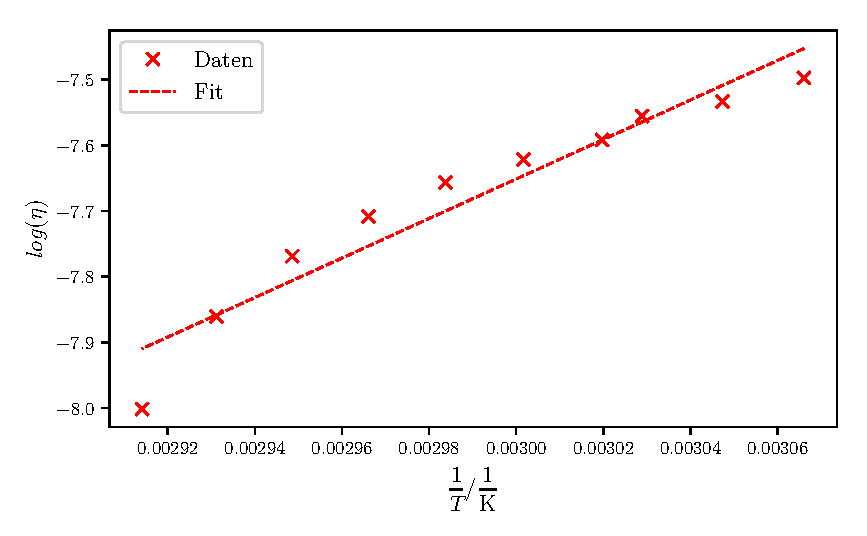
\includegraphics[width=14cm, height=10cm]{build/plot1.pdf}
    \caption{Die logarithmierte Viskosität ist gegen das Inverse
    der Falldauer der ersten Messung aufgetragen. Die Parameter
    aus Gleichung \eqref{eqn:temp} sind $A_1=\SI{0.566(515)}{\nano\pascal\second}$
    und $B_1=\SI{3012.12 \pm 304.10}{\kelvin}$.}
    \label{fig:plot1}
\end{figure}

\begin{figure}
    \centering
    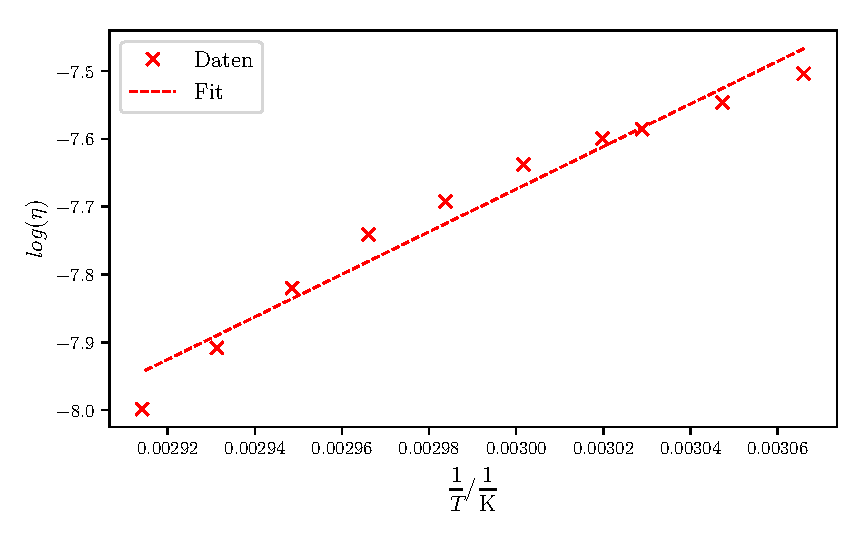
\includegraphics[width=14cm, height=10cm]{build/plot2.pdf}
    \caption{Die logarithmierte Viskosität ist gegen das Inverse
    der Falldauer der zweiten Messung aufgetragen. Die Parameter
    aus Gleichung \eqref{eqn:temp} sind $A_2=\SI{0.376(251)}{\nano\pascal\second}$
    und $B_2=\SI{3140.87 \pm 223.67}{\kelvin}$.}
    \label{fig:plot2}
\end{figure}

\subsection{Bestimmung der Reynoldszahlen}
Die Geschwindigkeit der kleinen Kugel ergibt sich mit Gleichung \eqref{eqn:v}
und der Falldauer $t_\text{klein}$ zu
\begin{equation*}
    v_\text{klein} = \SI{8.58(08)}{\milli\meter\per\second}.
\end{equation*}
Mit Gleichung \eqref{eqn:Re} folgt für die Reynoldszahl für die kleine Kugel
\begin{equation*}
    Re_\text{klein} = \num{172.7 \pm 3.1}.
\end{equation*}
Die Geschwindigkeit der großen Kugel ist
\begin{equation*}
    v_\text{groß} = \SI{1.534(007)}{\milli\meter\per\second}.
\end{equation*}
Die Reynoldszahl für die große Kugel ergibt sich auf die gleiche Weise zu
\begin{equation*}
    Re_\text{groß} = \num{31.27 \pm 0.31}.
\end{equation*}

\noindent Die Reynoldszahlen für die große Kugel bei verschiedenen Temperaturen ergeben sich auf die gleiche Weise und sind in folgender Tabelle aufgetragen. 
\begin{table}\caption{Die Temperatur und die Reynoldszahlen der erste und zweite Messung.}
\label{tab7}
\centering
\sisetup{round-mode = places, round-precision=2, round-integer-to-decimal=true}
\begin{tabular}{S[]S[]S[]} 
\toprule
{$T /\si{\kelvin}$} & {$Re_1$} & {$Re_2$}\\
\midrule
326.15 & 60.8+/-0.6 & 61.6+/-0.6\\
328.15 & 65.3+/-0.6 & 67.2+/-0.7\\
330.15 & 68.3+/-0.7 & 72.6+/-0.7\\
331.15 & 73.4+/-0.7 & 74.6+/-0.7\\
333.15 & 78.0+/-0.8 & 80.5+/-0.8\\
335.15 & 83.6+/-0.8 & 89.8+/-0.9\\
337.15 & 92.7+/-0.9 & 98.9+/-1.0\\
339.15 & 104.8+/-1.0 & 116.0+/-1.2\\
341.15 & 125.7+/-1.3 & 138.3+/-1.4\\
343.15 & 166.7+/-1.7 & 165.7+/-1.6\\
\bottomrule
\end{tabular}\end{table}


